\documentclass[10pt, a4paper, oneside, titlepage]{scrartcl} % article hat kein subtitle
\usepackage[utf8]{inputenc}
\usepackage{mathpazo}
\usepackage{setspace}
\usepackage{lscape}
\setstretch{1.3}
\usepackage{fancyhdr}
\pagestyle{fancyplain}
\fancyhead{}
\chead{\textbf{\leftmark{}}}
\cfoot{}
\rfoot{ \thepage{}}
\renewcommand{\headrulewidth}{0.8pt}
\usepackage{sectsty}
\sectionfont{\hspace{10pt}}
\subsectionfont{\vspace{30pt}}
\subsubsectionfont{\vspace{30pt}}
\usepackage[labelsep=colon, font=small, labelfont=bf]{caption}
\usepackage[pdftex]{graphicx}
\graphicspath{{img/}}
\usepackage[pdftex]{color}
\usepackage{colortbl}
\usepackage{parskip}
\usepackage[ngerman]{babel}
\usepackage{longtable}
\usepackage{pdfpages}

\usepackage[colorlinks, linkcolor = black, citecolor = black, filecolor = black, urlcolor = blue]{hyperref} 

\date{14. Januar 2014}
\hyphenation{Auf-sichts-rat Com-piler}
\author{Björn Ahlfeld, Patrick Borck, Jens Grundmann,\\ Sebastian Lun, Daniel Pinkpank, Phillippe Wels}
\title{LIAR - Lügendetektor}
\subtitle{Semesterprojekt im Fach Mobile Applications for Public Health}
\frenchspacing{} 
%-------------------------------------------------------------------
\begin{document}
   	\maketitle
   	\thispagestyle{empty}
	\tableofcontents
	\listoffigures
	\listoftables	
	   	\newpage   	
   	\section{Projektplanung}
	Im Folgenden sollen die Zielsetzung des Projektes Liar und die dafür notwendigen Meilensteine erläutert werden. Ferner wird eine fiktive Zeitungsmeldung mit einer Vision des Produktes, sowie eine fiktive Produktverpackung vorgestellt.
   	
   	\subsection{Zielsetzung}
   	Zielsetzung des Projektes Liar ist es, eine Smartphone Applikation zu entwickeln. Liar ist ein Gesellschaftsspiel auf Basis eines Lügendetektors und wird für das mobile Betriebssystem Android entwickelt. Im Spielverlauf stellt ein Nutzer A einem anderen Nutzer B Fragen. Nutzer B beantwortet diese Fragen, während er an zwei Sensoren angeschlossen ist. Dabei wird mittels eines EEG-Sensors und eines Galvanic Skin Sensors die Anspannung des antwortenden Nutzers evaluiert. Im Anschluss untersucht die LIAR App den Wahrheitsgehalt der Antwort des Nutzers und ordnet diesen dann in die Kategorien Lüge oder Wahrheit ein. Ferner ist es möglich sich sich sein EEG und auch den Hautleitwiderstand grafisch anzeigen zu lassen, sowie Informationen zur Interpretation der Messwerte in einer Hilfe nachzulesen.
   	
   	\newpage
   	\subsection{Meilensteine}
	Meilensteine repräsentieren Zwischenergebnisse in der Programmentwicklung die von besonderer Bedeutung sind. Sie eignen sich zur Arbeitsaufteilung in einer Gruppe.
	\subsubsection{Einarbeitung}
	\begin{itemize}
	\item{}Android SDK installieren
	\item{}Android Tutorial absolvieren
	\item{}Einarbeitung in Mindwave Mobile (EEG-Sensor)
	\item{}Einarbeitung in das SDK des Galvanic Skin Sensors
	\end{itemize}	  	
	\subsubsection{Aufbau eines User Interfaces}
	\begin{itemize}
	\item{}Hauptbildschirm mit den Elementen(neues Spiel starten, Eigenanalyse, Ranglisten und Spielanleitung)
	\item{}Spielstartbildschirm auf dem die Anzahl der zu spielenden Runden, die Anzahl der Spieler und deren Namen eingetragen werden können.
	\item{}Eigenanalysebildschirm: zeigt die Messwerte beider Sensoren in zwei Graphen an und erlaubt eine Aufzeichnung von Daten, eine Ansicht älterer Daten, sowie zwei Informationsbuttons mit Wissenswerten Informationen zum EEG und Galvanic Skin Sensor
	\item{}Auswertungsbildschirm: zeigt das Ergebnis der Fragerunde (Anzahl der wahrheitsgemäß beantworteten Fragen, Anzahl der vermeintlich nicht wahrheitsgemäß beantworteten Fragen, Batch-System für das Erreichen einer besonderen Leistung [z.B. ehrliche Haut oder Lügner des Monats])
	\end{itemize}
	\subsubsection{Anbindung des EEG Sensors}
	\begin{itemize}
	\item{}Einrichtung einer Bluetoothverbindung zum EEG-Sensor
	\item{}Auslesen der Daten des EEG-Sensors
	\item{}Interpretieren der Daten des EEG-Sensors
	\item{}grafische Darstellung der Daten des EEG-Sensors
	\end{itemize}
	\subsubsection{Anbindung des Galvanic Skin Sensors}
	\begin{itemize}
	\item{}Einrichtung einer Bluetoothverbindung vom Arduino Shield zum Galvanic Skin Sensor
	\item{}Einrichtung einer Bluetoothverbindung vom Smartphone zum Arduino Shield
	\item{}Auslesen der Daten der Messdaten
	\item{}Interpretieren der Messdaten
	\item{}grafische Darstellung der Messdaten
	\end{itemize}
   	

	\newpage
   	\subsection{fiktive Zeitungsmeldung}
   	Die folgende fiktive Zeitungsmeldung stellt aus Sicht der Entwickler die Perspektiven und Erwartungen an das LIAR Projekt dar. 
	\begin{figure}[ht!]
		\begin{center}
			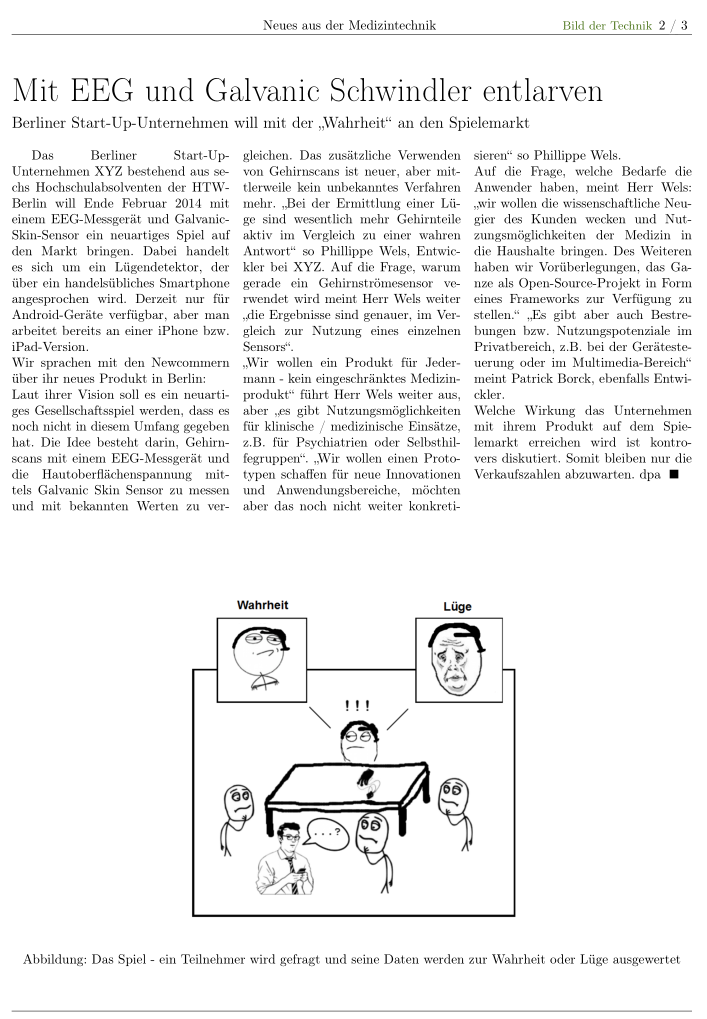
\includegraphics[width=0.8\textwidth]{zeitungsmeldung.png}
		\end{center}
		\caption[Zeitungsmeldung]{fiktive Zeitungsmeldung}
	\label{fig:zeitungsmeldung}
	\end{figure}   

	%\includepdf[pagecommand={\thispagestyle{fancy}}, pages=2, scale=0.55, frame=true]{pdf/zeitungsmeldung.pdf}   

   	\subsection{Produktverpackung}
   	Die folgende Abbildung stellt die auf die Nutzergruppe angepasste Produktverpackung der LIAR-App dar.
	\begin{figure}[ht!]
	\begin{center}
		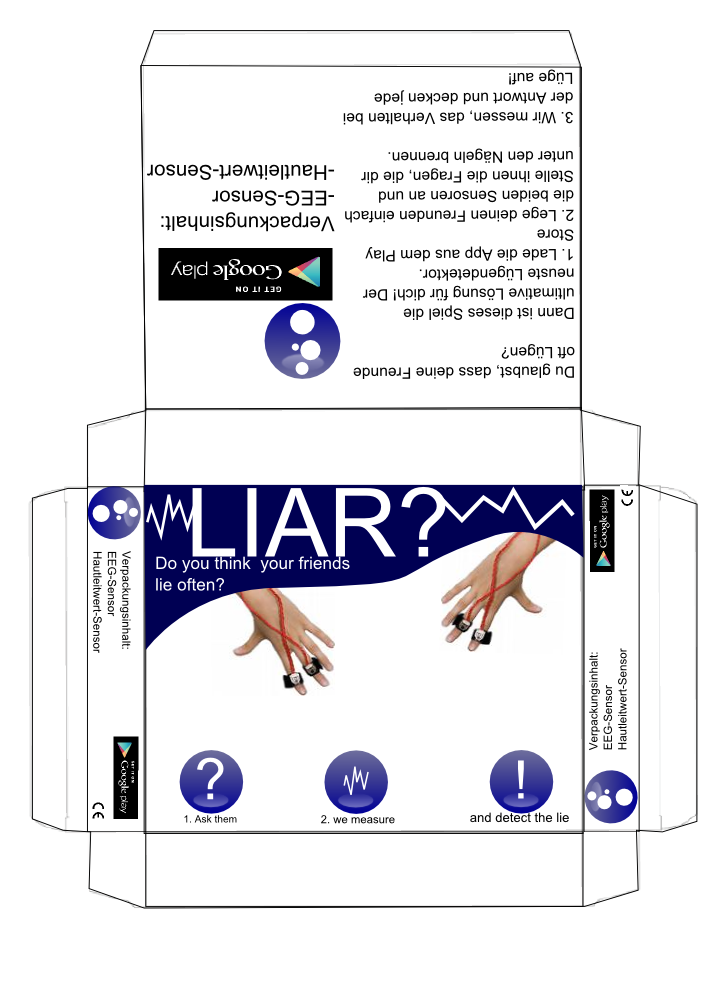
\includegraphics[width=0.8\textwidth]{verpackung.png}
	\end{center}
	\caption[Produktverpackung]{Produktverpackung Liar Android App}
	\label{fig:verpackung}
	\end{figure}   
   
	   	\newpage
   	\section{Personas und Anwendungsszenarien}
   	Dieses Kapitel befasst sich mit Personas und deren Anwendungsszenarien. Eine Persona ist eine Person, die eine Gruppe von zukünftigen Nutzern der Applikation beispielhaft repräsentiert. Personas haben konkrete Eigenschaften und zeigen in einem Anwendungsszenario, wie sie mit dem Produkt umgehen wollen.
   	
	\subsection{Persona 1 - ,,Der Kontrollfreak'': Elisa Schubert (20)}
	\begin{center}
		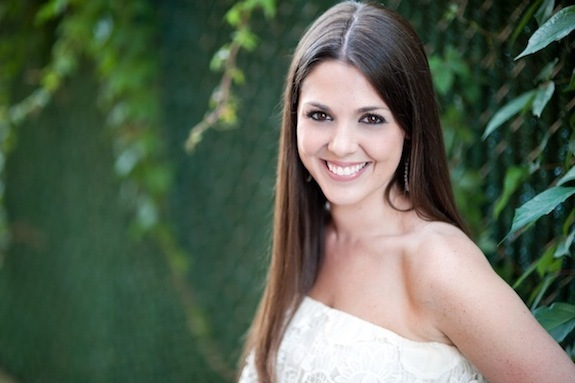
\includegraphics[width=0.7\textwidth]{persona_01.jpg}
	\end{center}
	\subsubsection{Soziodemografische Daten}
	Elisa Schubert ist 20 Jahre alt. Sie ist ledig und zur Zeit in einer festen Beziehung. Vor einem Jahr hat sie ihr Abitur gemacht. Aktuell studiert sie die Fächer Deutsch und Biologie an der Universität zu Köln.
	\subsubsection{Vorlieben, Hobbys, Abneigungen}
	Frau Schubert singt in einem Gospel-Chor, geht gern auf Partys und engagiert sich in ihrer Freizeit ehrenamtlich bei der Naturschutzorganisation WWF. Sie ist notorisch eifersüchtig auf jede Frau, die sich Ihrer Jugendliebe Bernd nähert. Da Bernd auch dafür bekannt ist, ,,mehrgleisig'' unterwegs zu sein, will sie immer wieder Gewissheit, dass er nur sie liebt. Frau Schubert hasst es belogen zu werden. Sie ist ein Kontrollfreak und liest heimlich die SMS von Bernd. Für ihre Zukunft hat sich Elisa vorgenommen, mit Bernd eine Familie gründen und Ihr Studium erfolgreich zu beenden. 
	\subsubsection{Nutzererwartung an das Produkt}
	Elisa ist neugierig was andere Menschen, insbesondere ihre Freunde, über sie denken. Sie erwartet von der LIAR App, dass sie Bernd besser kontrollieren kann und erhofft sich Einblicke in die verborgene Gedankenwelt ihrer Freunde.
	\subsubsection{Anwendungsszenario}
	An einem gemütlichen Samstag Abend spielen Elisa, Bernd und einige Freunde Karten- und Gesellschaftsspiele. Elisa hat die LIAR App, samt den dazugehörenden Sensoren mitgebracht und stellt sie ihren Freunden vor. So ist sie in der Lage auf unauffällige Art und Weise Bernd Fragen zu stellen und seine Antworten auf den Wahrheitsgehalt hin zu überprüfen. Die anderen Freunde stellen einander ebenfalls Fragen und haben dabei viel Spaß.
   
   	\subsection{Persona 2 - ,,Der Wissenschaftler'': Frank Bollwerker (36)}
   	\begin{center}
		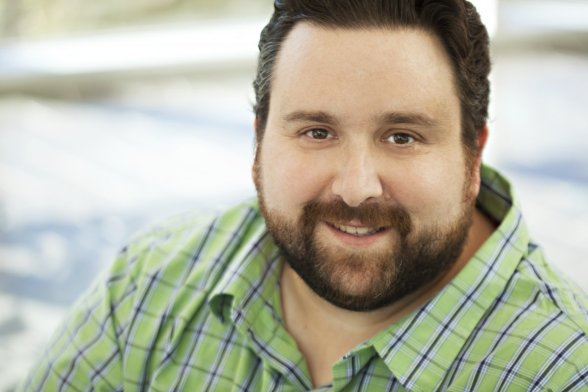
\includegraphics[width=0.7\textwidth]{persona_02.jpg}
	\end{center}
	\subsubsection{Soziodemografische Daten}
	Frank Bollwerker ist 36 Jahre alt, verheiratet und zur Zeit noch kinderlos. Er hat sein Physikstudium abgeschlossen und arbeitet seit dieser Zeit als wissenschaftlicher Mitarbeiter im Studiengang Luft- und Raumfahrttechnik an der Universität Stuttgart.
	\subsubsection{Vorlieben, Hobbys, Abneigungen}
	Frank ist ein gewissenhafter Forscher, der seit einem halben Jahr nach einem passenden Thema für seine Doktorarbeit sucht. Er überlegt, ob er erweiterte Tests zur Auswahl der zukünftigen Raumfahrer entwickeln sollte, welche neben den kognitiven und körperlichen Aspekten auch den Wahrheitswert von Antworten auf Fragen untersucht. Frank spielt in seiner Freizeit Bowling und geht gerne Wandern.
	\subsubsection{Nutzererwartung an das Produkt}
	Herr Bollwerker erwartet ein Produkt, was höchsten wissenschaftlichen Ansprüchen gerecht wird. Er erhofft sich mit der LIAR App signifikante und eindeutige Aussagen zu den Antworten von zukünftigen Raumfahrern zu erhalten.
	\subsubsection{Anwendungsszenario}
	Während der Fahrt mit den öffentlichen Verkehrsmitteln zu Universität findet Herr Bollwerker die LIAR-App im Google Play Store und beliest sich zum Thema Lügendetektor. Er beschließt die App zu kaufen und auf Verwendbarkeit für seine wissenschaftliche Arbeit zu testen.
	
	\subsection{Persona 3 - ,,Der Angeber'': Jonas Keppler (29)}
	\begin{center}
		
\includegraphics[width=0.7\textwidth]{persona_03.jpg}
	\end{center}
	\subsubsection{Soziodemografische Daten}
	Jonas Keppler ist 29 Jahre alt und ledig. Eine feste Freundin hat nicht, da diese wie die Hemden wechselt. Er nach seinem Germanistikstudium eine Journalistenschule in Bonn besucht. Nebenbei hat er in einem kleinen Softwareunternehmen als Webentwickler gearbeitet um seinen monatlichen Ausgaben zu decken. Seit 6 Monaten arbeitet als Redakteur im Ressort "Digital" bei der Süddeutschen Zeitung in München.
	\subsubsection{Vorlieben, Hobbys, Abneigungen}
	Herr Keppler ist sehr interessiert an neuer Technik und coolen Apps, die er dann stolz während der Mittagspause all seinen Arbeitskollegen präsentiert. Er 	steht gern im Mittelpunkt. Jeden Donnerstag geht ins Kino und schaut sich die neuesten Filme in der Sneak Preview an. Er immmer der Erste, der etwas Neues ausprobiert. Jonas Keppler macht Yoga und achtet sehr auf seine Ernährung. Er kauft im Biomarkt ein und wird im nächsten Sommer erstmals selbst Gemüse auf seinem Grundstück anbauen.
	\subsubsection{Nutzererwartung an das Produkt}
	Jonas erwartet ein Produkt, was sich als Publikumsmagnet für die nächste WG-Party eignet. Es muss andere Leute neugierig machen und sollte ihn als Entertainer dastehen lassen. 
	\subsubsection{Anwendungsszenario}
	Jonas Keppler im Internet von der LIAR-App gelesen und war der Erste, der sich den Prototyp bestellt hat. Den nächsten Werktag kann er gar nicht mehr abwarten, denn er weiß, dass ihm die Aufmerksamkeit der Kollegen damit gewiss ist.
	
	   	\section{Anforderungen}
   	Im Folgenden Abschnitt werden die Anforderungen für die LIAR Android App aufgelistet.
   	
   	\subsection{Muss-Kriterien}
	\begin{itemize}
	\item{}Die App soll mit dem mobilen Betriebssystem Android entwickelt werden.
	\item{}Ein EEG- und eine Galvanic Skin Sensor (Hautleitwert) sollen Daten an das Android Smartphone senden können.
	\item{}Die Messwerte des EEG-Sensors und der Hautleitwert des Benutzers sollen auf dem Smartphone ausgelesen werden können.
	\item{}Die Messwerte des Benutzers können ausgewertet und angezeigt werden.
	\item{}Es kann ein Benutzerprofil erstellt werden.
	\item{}Es lässt sich eine neue Spielsession (Spielsession, Spieldauer, Spieleranzahl) erstellen.
	\item{}Das Speichern der Messwertauswertung je Benutzer ist möglich.
	\item{}Eine Spielsession kann durchgeführt werden.
	\item{}Es kann ein Lügendetektortest mit vorgegebenen Fragen absolviert werden.
 werden.
	\item{}Die Spielergebnisse werden angezeigt und können gespeichert werden.
	\end{itemize}		
	
	\subsection{Kann-Kriterien}
	\begin{itemize}
		\item{}Die Anzeige der Messwerte des EEG-Sensors und der Hautleitwert des Benutzers soll grafisch in einem dynamischen XY-Diagramm erfolgen.
		\item{}Es kann ein Lügendetektortest mit eigenen Fragen absolviert werden.
		\item{}Die Spielergebnisse können auf sozialen Netzwerken veröffentlicht werden.	
	\end{itemize}

	
		\newpage	
	\section{priorisierte User Stories}	
	\subsection{User Stories mit hoher Priotität:}
	\begin{itemize}
	\item{}Der Anwender kann das Spiel über eine Smartphone-App öffnen.
	\item{}Der Anwender kann seinen Messwert sehen und speichern.
	\end{itemize}
	\subsection{User Stories mit mittlerer Priorität:}
	\begin{itemize}
	\item{}Ein Gast muss sich registrieren können	
	\item{}Der Anwender kann Text eingeben, um einen Fragenkatalog zu erstellen.
	\item{}Anwender kann für das Spiel die Anzahl der Mitspieler und Fragen einstellen.
	\item{}Spieler erkennen Lüge oder Wahrheit nachdem eine Frage beantwortet wurde.
	\end{itemize}
	\subsection{User Stories mit niedriger Priorität:}
	\begin{itemize}
	\item{}Der Anwender soll die Anzahl der  Mitspieler auswählen können.
	\item{}Jeder Mitspieler kann seinen Punktestand einsehen.
	\item{}Über ein Leaderboard ist es möglich sich mit anderen Spielern zu messen.
	\item{}Anwender können ihren Punktestand via Facebook teilen.
	\item{}Anwender kann Fragen beantworten.
	\item{}Gespeicherte Fragerunden können nochmal gespielt werden.
	\end{itemize}

		\begin{landscape}
   	\section{Risikobetrachtung}
   	\begin{table}[h!]
		\begin{center}
			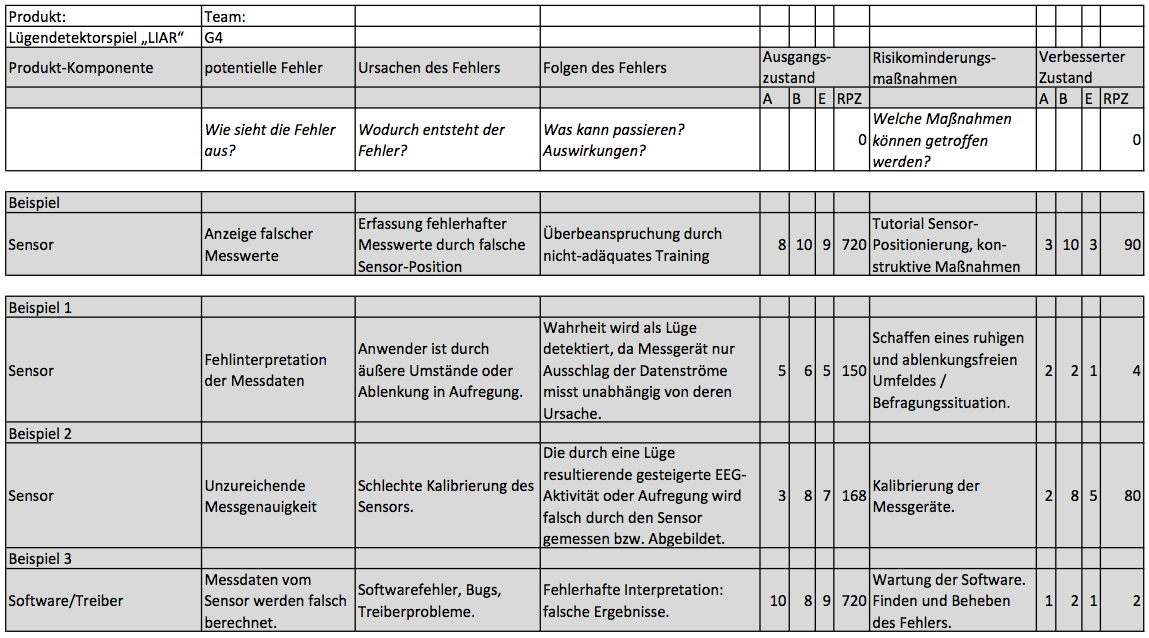
\includegraphics[width=1.3\textwidth]{risikobetrachtung.png}
		\end{center}
		\caption[Risikoanalyse]{Risikoanalyse}
		\label{fig:risikoanalyse}
	\end{table}
	\end{landscape}

	   \newpage
   \section{Systemüberblick und Systemarchitektur}
   Im Folgenden soll ein Überblick der verwendeten Systemkomponenten gegen werden. In Abbildung 2 ist der generelle Ablauf der Kommunikation zwischen den Komponenten dargestellt. Die emotionale Erregung des Nutzers soll über zwei Sensoren gemessen werden. Zum einen erfolgt eine Messung des elektrischen Widerstandes der Haut über einen Galvanic Skin Sensor. Der Galvanic Skin Sensor kommuniziert über eine Bluetooth-Verbindung mit einem Arduino Shield. Das Arduino Shield wiederum ist via Bluetooth mit dem Smartphone des Nutzers verbunden. Der zweite Sensor ermöglicht die Registrierung der Hirnströme und wird als  Elektroenzephalografie, kurz EEG, bezeichnet. Der EEG-Sensor kommuniziert ebenfalls über das Bluetooth-Protokoll mit dem Smartphone. Im Smartphone werden die vom Nutzer gewonnenen Daten ausgewertet und verständlich dargestellt. Messergebnisse können zum einen lokal in einer Datenbank abgelegt werden oder auch mit anderen Freunden auf einer Social Media Plattform geteilt werden.
   	\begin{figure}[ht!]
		\begin{center}
			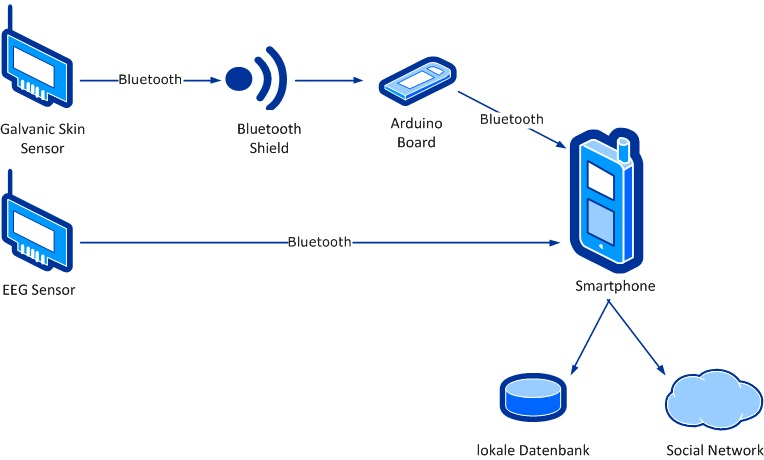
\includegraphics[width=0.9\textwidth]{systemarchitektur_01.jpg}
		\end{center}
		\caption[Systemarchitektur]{Systemarchitektur}
		\label{fig:system1}
	\end{figure}	
	
		\newpage
   	\section{Entwurf / Mockup des User-Interface}

	\begin{figure}[ht!]
		\begin{center}
			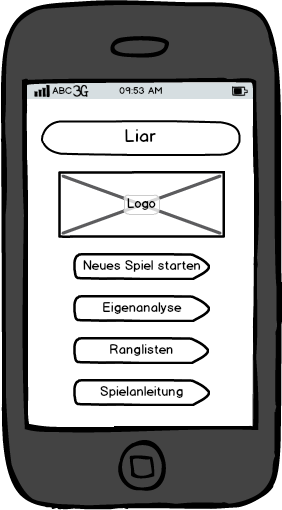
\includegraphics[width=0.3\textwidth]{mockup_01_index.png}
		\end{center}
		\caption[Mockup Hauptbildschirm]{Der Hauptbildschirms der LIAR-App umfasst die Menüpunkte: neues Spiel starten, Eigenanalyse, Ranglisten sowie Spielanleitung. }
		\label{fig:mockup_01}
	\end{figure}	
	\begin{figure}[h!]
		\begin{center}
			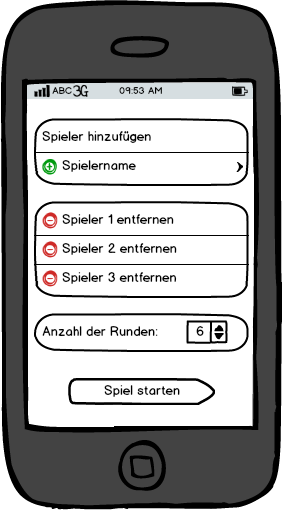
\includegraphics[width=0.3\textwidth]{mockup_02_newgame.png}
		\end{center}
		\caption[Mockup Bildschirm für neues Spiel]{Der Bildschirm für ein neues Spiel erlaubt das Festlegen der Spielernamen, der Spieleranzahl und der zu spielenden Runden.}
		\label{fig:mockup_02}
	\end{figure}	

	\newpage
	\begin{figure}[ht!]
		\begin{center}
			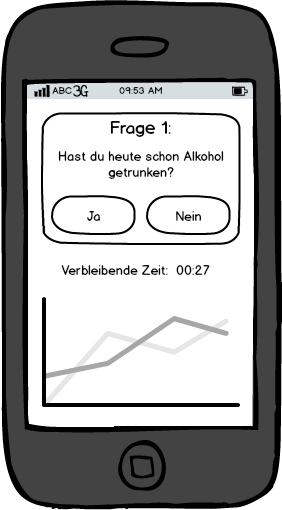
\includegraphics[width=0.3\textwidth]{mockup_03_playgame.png}
		\end{center}
		\caption[Mockup Spielbildschirm]{Der Spielbildschirm zeigt eine Frage, deren Antwortmöglichkeiten, die verstrichene Zeit, sowie den grafischen Verlauf der Sensordaten.}
		\label{fig:mockup_03}
	\end{figure}	
	\begin{figure}[h!]
		\begin{center}
			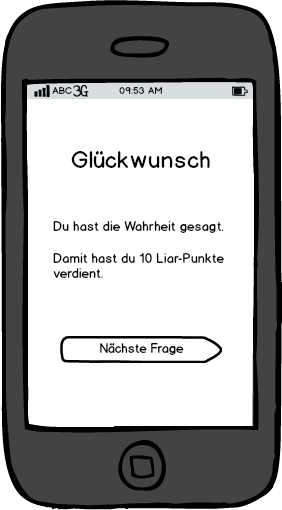
\includegraphics[width=0.3\textwidth]{mockup_04_score.png}
		\end{center}
		\caption[Mockup Bildschirm Fragenauswertung Wahrheit]{Auswertungsbildschirm bei wahrheitsgemäßer Antwort}
		\label{fig:mockup_04}
	\end{figure}	

	\newpage
	\begin{figure}[ht!]
		\begin{center}
			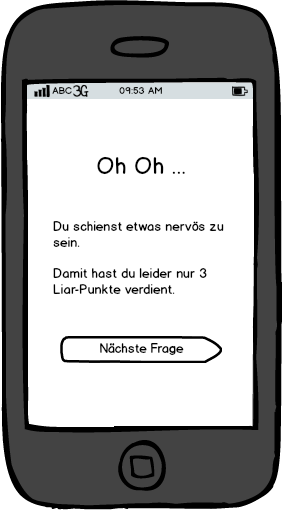
\includegraphics[width=0.3\textwidth]{mockup_05_score2.png}
		\end{center}
		\caption[Mockup Bildschirm Fragenauswertung Lüge]{Auswertungsbildschirm bei nicht wahrheitsgemäßer Antwort}
		\label{fig:mockup_05}
	\end{figure}	
	\begin{figure}[h!]
		\begin{center}
			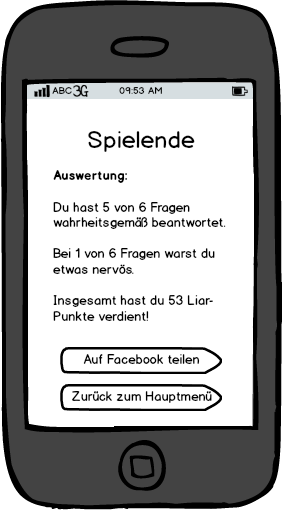
\includegraphics[width=0.3\textwidth]{mockup_06_finalscore.png}
		\end{center}
		\caption[Mockup finaler Bildschirm zur Fragenauswertung]{finaler Auswertungsbildschirm eines Spiels}
		\label{fig:mockup_06}
	\end{figure}	

	\newpage
	\begin{figure}[ht!]
		\begin{center}
			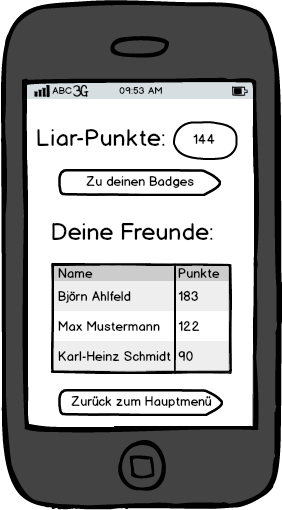
\includegraphics[width=0.3\textwidth]{mockup_07_ranking.png}
		\end{center}
		\caption[Mockup highscore-Bildschirm]{Der Ranking-Bildschirm zeigt die highscore-Einträge der Spieler}
		\label{fig:mockup_07}
	\end{figure}	
	\begin{figure}[h!]
		\begin{center}
			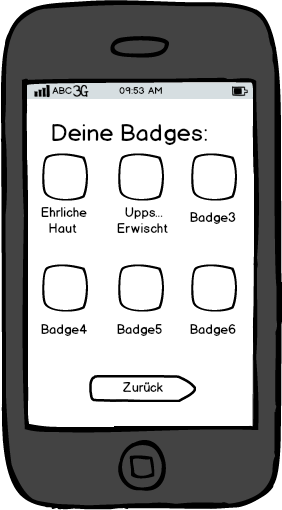
\includegraphics[width=0.3\textwidth]{mockup_08_badges.png}
		\end{center}
		\caption[Mockup Badge-Bildschirm]{Der Bildschirm zeigt das Badge-System, bei dem Spieler für bestimmte Leistungen Auszeichnungen erhalten.}
		\label{fig:mockup_08}
	\end{figure}	

	\newpage
	\begin{figure}[ht!]
		\begin{center}
			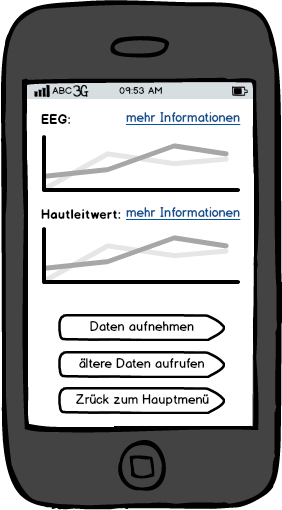
\includegraphics[width=0.3\textwidth]{mockup_09_selfanalysis.png}
		\end{center}
		\caption[Mockup Bildschirm Eigenanalyse]{Der Eigenanalyse-Bildschirm veranschaulicht die Messwerte aller Sensoren,erlaubt das Abspeichern von Daten, den Zugriff auf alte Daten und bietet Hilfetexte zu den verwendeten Sensoren an.}
		\label{fig:mockup_09}
	\end{figure}	
	\begin{figure}[h!]
		\begin{center}
			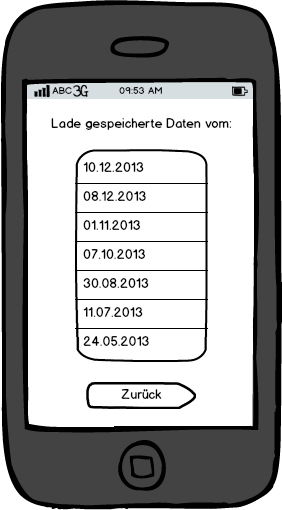
\includegraphics[width=0.3\textwidth]{mockup_10_saveddata.png}
		\end{center}
		\caption[Mockup Bildschirm zum Laden gespeicherter Daten]{Der Bildschirm zum Laden gespeicherter Daten erlaubt den Zugriff auf vergangene Eigenanalysen.}
		\label{fig:mockup_10}
	\end{figure}	
	
	\newpage
	\begin{figure}[ht!]
		\begin{center}
			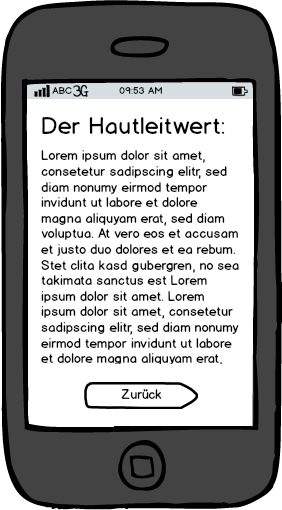
\includegraphics[width=0.3\textwidth]{mockup_11_skinconductance.png}
		\end{center}
		\caption[Mockup Infobildschirm Hautleitwert]{Der Informationsbildschirm Hautleitwert erklärt verständlich den genannten Sensor.}
		\label{fig:mockup_11}
	\end{figure}	
	\begin{figure}[h!]
		\begin{center}
			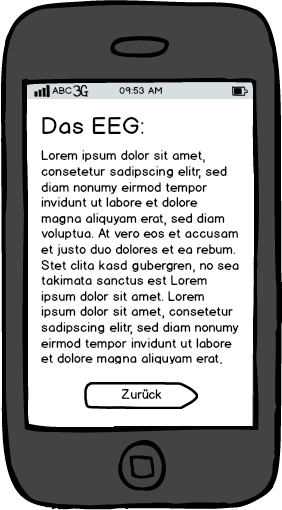
\includegraphics[width=0.3\textwidth]{mockup_12_eeg.png}
		\end{center}
		\caption[Mockup Infobildschirm EEG]{Der Informationsbildschirm EEG erklärt verständlich den genannten Sensor.}
		\label{fig:mockup_12}
	\end{figure}	

	\newpage
	\begin{figure}[ht!]
		\begin{center}
			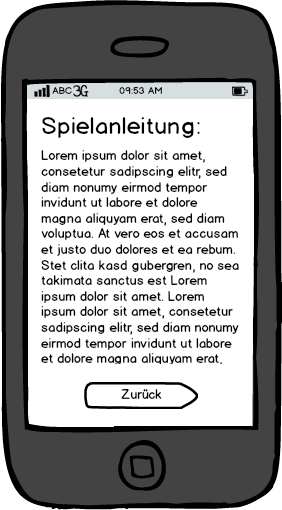
\includegraphics[width=0.3\textwidth]{mockup_13_instructions.png}
		\end{center}
		\caption[Mockup Anleitungsbildschirm]{Der Anleitungsbildschirm erklärt die wichtigsten Sachverhalte zu App und Sensoren.}
		\label{fig:mockup_13}
	\end{figure}	

   	%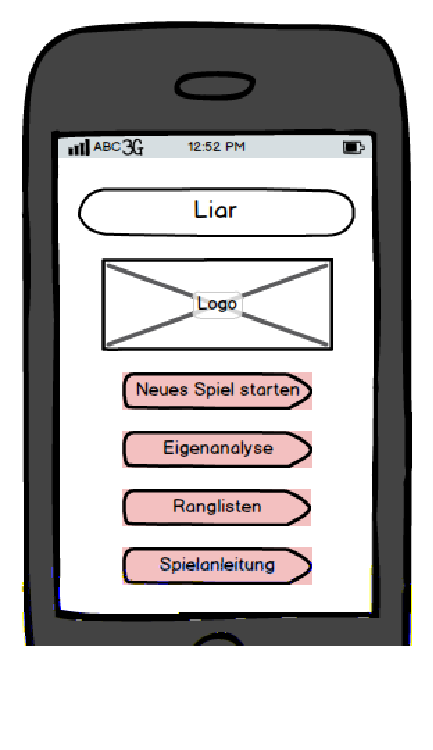
\includepdf[pagecommand={\thispagestyle{fancy}}, pages=1-13, scale=0.6, frame=true]{pdf/mockups.pdf}

	   	\newpage
	\section{Implementierungen}

	Das folgende Kapitel der \textit{Implementierungen} gibt einen Überblick über die verwendeten Technologien für das Produkt. Es werden genutzte (offene) Schnittstellen genannt, vorgestellt und deren Funktionsweise beschrieben. Zusätzlich werden selbst entwickelte Komponenten beschrieben und deren Implementierungen (sofern nötig) erörtert.
	
	\subsection{Arduino}
	
	Die Arduinoplattform ermöglicht eine \texttt{stackable}\footnote{aufeinderstecken verschiedener Module - vergleichbar mit Lego-Prinzip} Aneinanderkopplung verschiedener technischer Module. Unter anderem wurden in diesem Projekt ein e-Health-Modul, zum Auslesen von Galvanic Skin Daten, und zum Anderen die Anbindung an ein Wireless + Bluetooth Shield verwandt und eingesetzt. Die einzelnen Komponeten werden wie folgt beschrieben und durch die Beschreibung des Endprodukts vervollständigt.
		
	\subsubsection{eHealth - Plattform}
	
	Das e-Health-Modul ermöglicht es Android-Nutzer auf biometrische Daten zuzugreifen. Zu diesen Daten zählen unter anderem Puls-Messung, Blutdruck, EKG, Kör-pertemperatur und auch die Hautleitfähigkeit (GSR \^= galvanic skin response).

	Das e-Helath-Modul ist stackable und lässt sich daher einfach auf ein Arduino Uno ,,aufsetzen``. Hier ist darauf zu achten, dass es nicht zu verbogenen oder abgebrochenen Metall- / Verbindungsstücken kommt.
	
	\begin{figure}[hbtp]
	\centering
	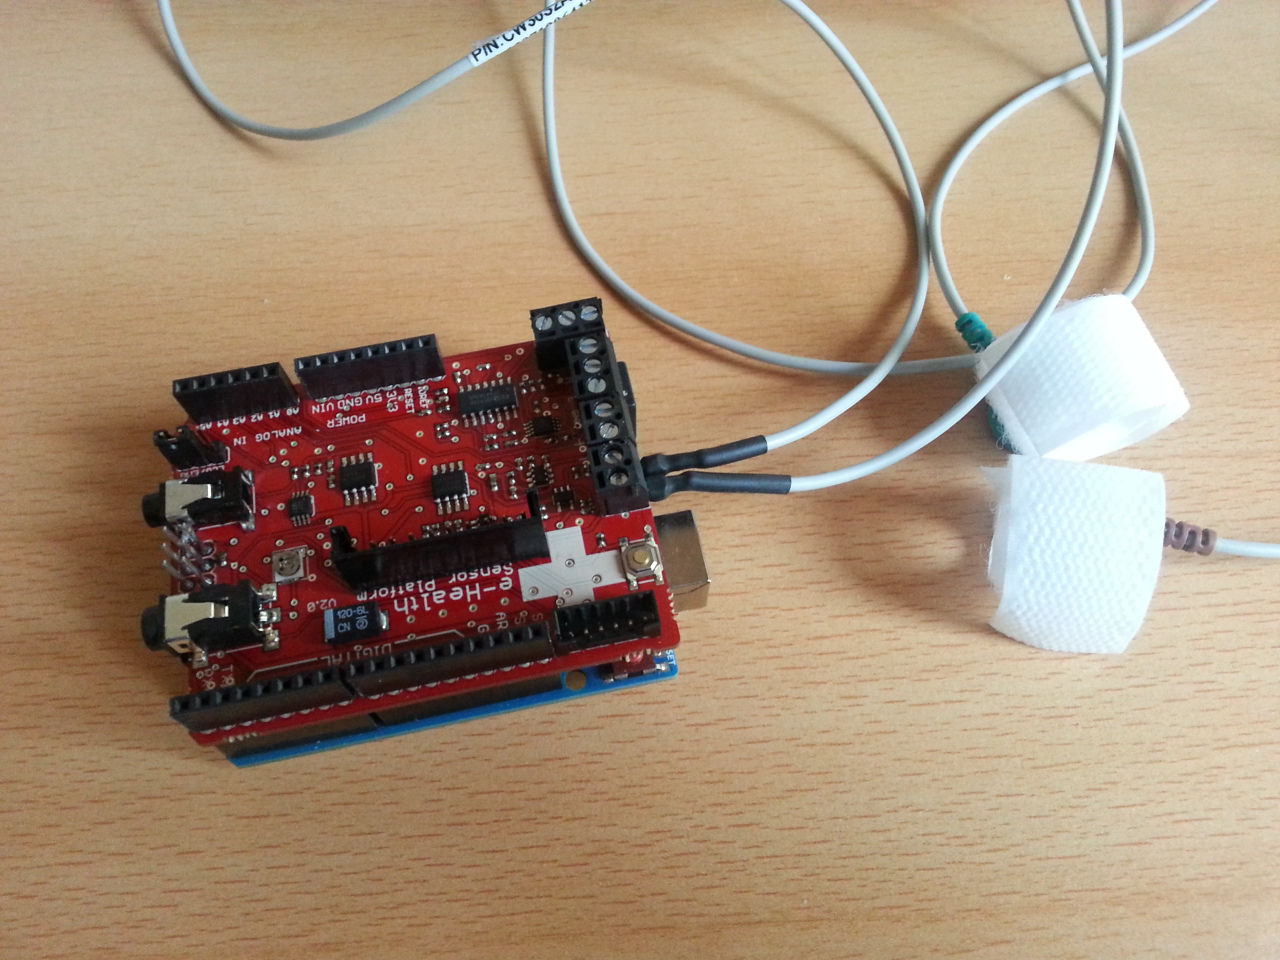
\includegraphics[width=0.7\textwidth]{implementierung_arduino+ehelath-modul.jpg}
	\caption{Arduino-eHealth-Stack}
	\label{fig:Arduino-eHealth-Stack}
	\end{figure}
	
	
	Zur Programmierung eines Arduino-Programms ist neben der Installation der entsprechenden Arduino IDE und der Treiberinstallation der Arduino Hardware, die entsprechenden e-Health Libraries herunterzuladen und unter dem Standardinstallationsordner der Arduino-IDE abzulegen, z.B.:
	\begin{itemize}
	\item \texttt{C:\textbackslash Arduino\textbackslash arduino-1.0.5\textbackslash libraries\textbackslash eHealth}
	\item \texttt{C:\textbackslash Arduino\textbackslash arduino-1.0.5\textbackslash libraries\textbackslash PinChangeInt}
	\end{itemize}
	
	Danach kann in der Arduino IDE das gewünschte Programm erstellt werden. Dazu sollte zuerst das e-Health Package eingebunden werden, dann kann man auf den / die gewünschten Sensor / -en zugreifen:
	
	\begin{enumerate}
	 \item \texttt{\#include $ <eHealth.h> $}
	 \item ...
	 \item \texttt{float resistance = $eHealth$.getSkinResistance();}
	 \end{enumerate} 
	 
	 Die Variable $resistance$ sollte in der loop-Funktion deklariert und definiert werden, um sicher zu stellen, dass die Werte immer ,,frisch`` in die Variable geschrieben werden.
	 
	 Für weitere Information zur e-Health-Plattform im besonderen zur GSR verweisen wir auf die \href{http://www.cooking-hacks.com/documentation/tutorials/ehealth-biometric-sensor-platform-arduino-raspberry-pi-medical\#step4\_7}{e-Health-Website}.
	
	\subsubsection{Wireless + Bluetooth Shield}
	
	Das Wireless + Bluetooth Shield es ebenfalls stackable und kann auf das Arduino Uno aufgesetzt werden. 
	Im folgenden Fall stand neben dem Wireless Shield das Zusatzmodul \texttt{BlueTooth Bee} von iteadstudio zur Verfügung. Das Bluetooth-Modul hatte die Spezifikation V2.0 und Modelbezeichnung HC-06. 
	
		\begin{figure}[hbtp]
		\centering
		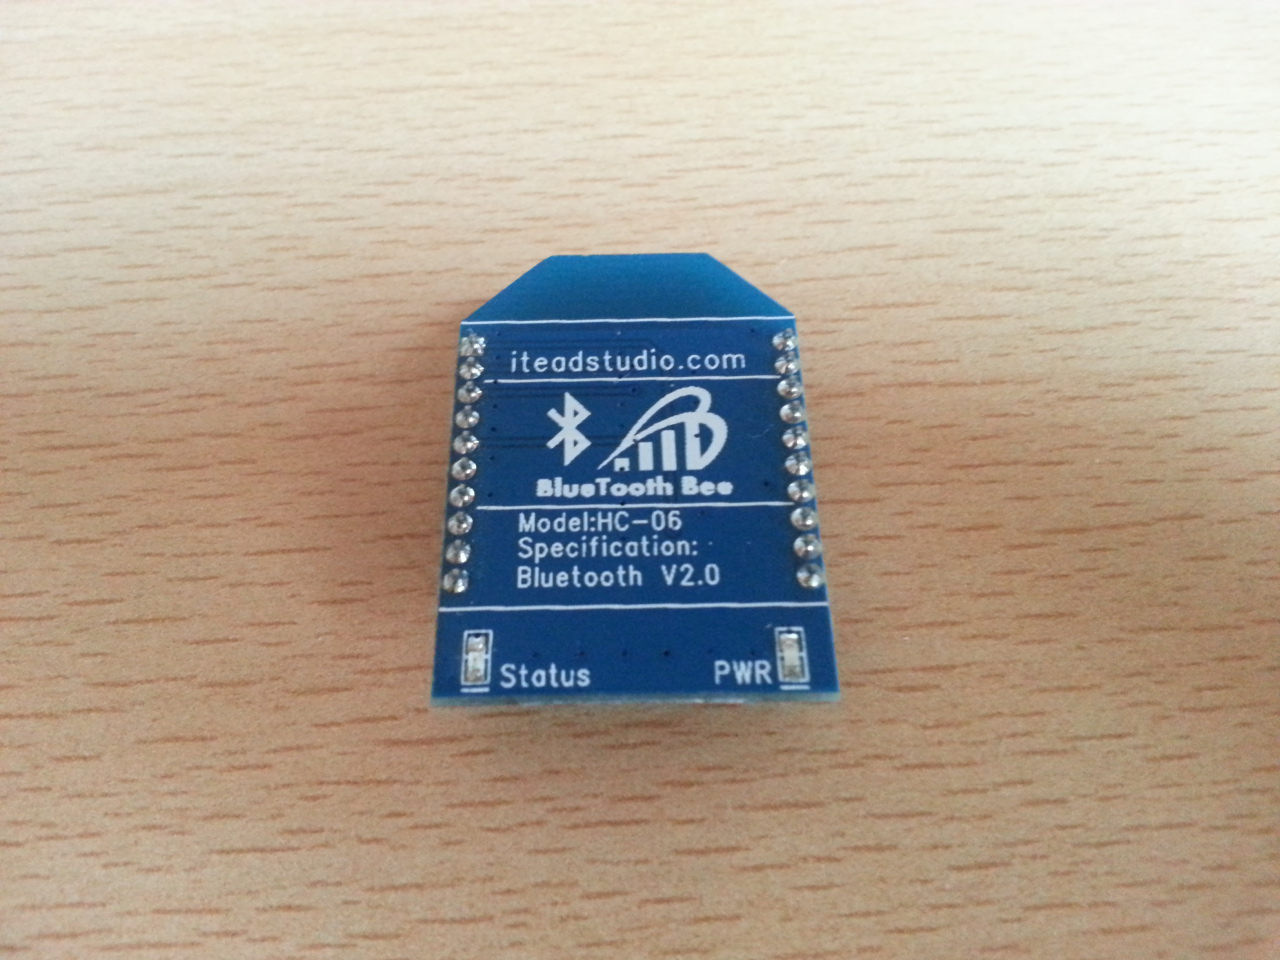
\includegraphics[width=0.7\textwidth]{implementierung_bluetooth-modul.jpg}
		\caption{Das Bluetooth Modul}
		\label{fig:Bluetooth-Modul}
		\end{figure}
		
	
	Die Modelbezeichnung ist ausschlaggebend dafür, ob ein solches Modul im Master\footnote{kann aktives Pairing zu anderen Geräten übernehmen (Serverfunktionalität)}, Master+Slave oder nur Slave\footnote{kann kein Pairing übernehmen} Modus arbeitet. In diesem Fall bestand mit diesem Modul die einfache Slave-Funktionalität zur Verfügung.
	
	\begin{figure}[hbtp]
	\centering
	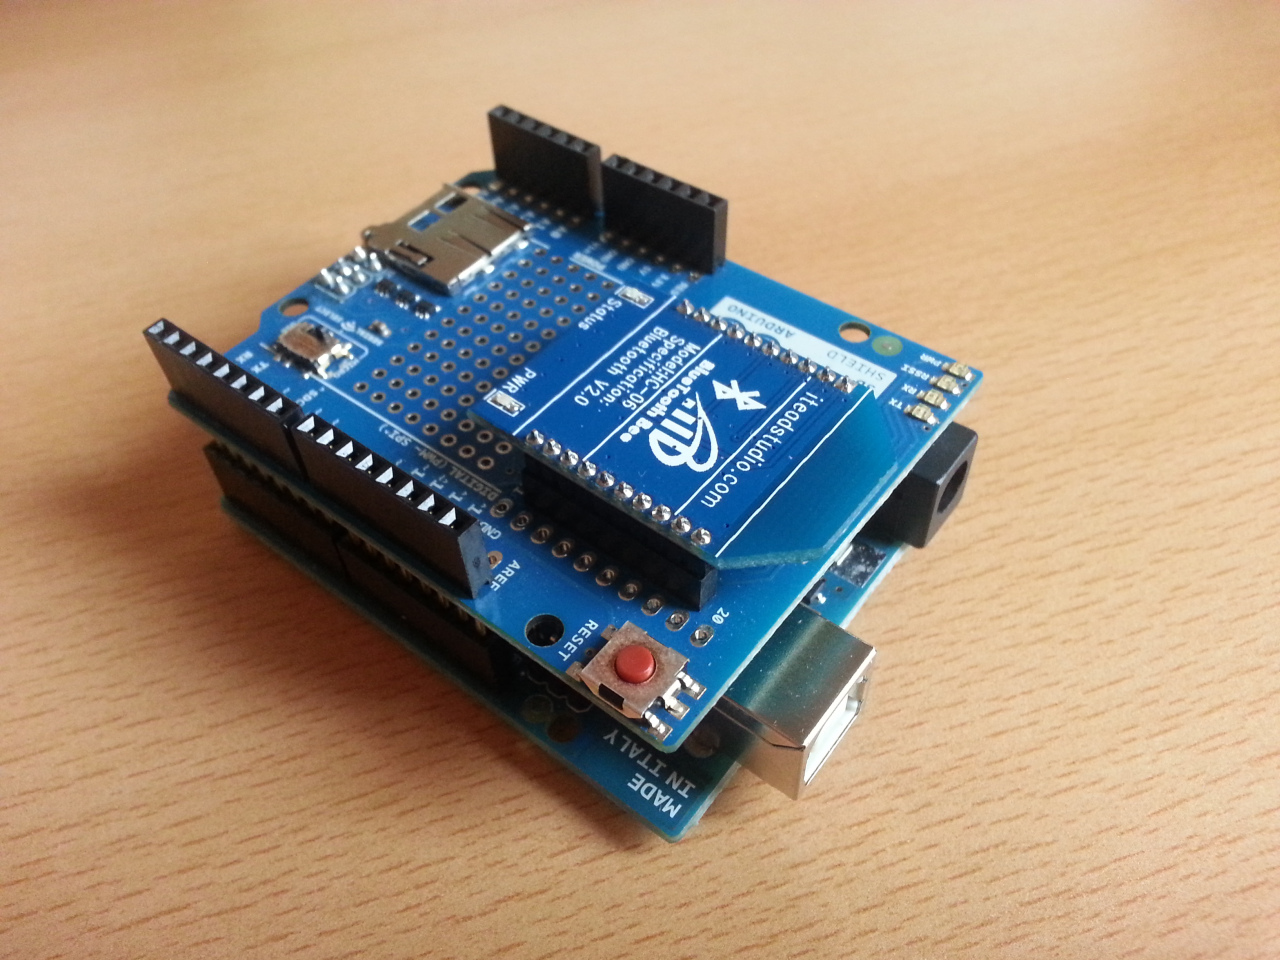
\includegraphics[width=0.7\textwidth]{implementierung_arduino+wireless-shield.jpg}
	\caption{Der Ardunio-Bluetooth-Stack}
	\label{fig:Arduino-Bluetooth-Stack}
	\end{figure}
	
	Die Implementierung der Bluetooth-Verbindung läuft im Slave-Modus über die serielle Verbindung. Dazu wird im Setup ein \texttt{Serial.begin($<baud\_rate>$)} aufgerufen. Die Baudrate richtet sich nach der Übertragungsgeschwindigkeit mit der das Bluetooth-Modul arbeiten soll und mit der die entsprechende Gegenstation (Master) arbeitet. 
	
	In der $loop()$-Funktion ist dann der entsprechende zu übertragende Wert mit \\$Serial.print(<value>)$ über die serielle Schnittstelle auszugeben. Zusätzlich ist nach jedem Wert die Zeichnkette ,,\textbackslash r\textbackslash n'' mit $Serial.print();$ zu übergeben. Sie signalisiert den Abschluss eines Datensatzes.
	
	
	\subsubsection{Endprodukt}

	Beim Zusammenfügen der einzelnen Komponenten musste die Reihenfolge:
	\begin{itemize}
	\item Oben: Wireless + Bluetooth - Shield
	\item Mitte: e-Health-Modul
	\item Unten: Arduino Uno
	\end{itemize}
	
	eingehalten werden, da sonst das e-Health-Modul nicht mit Strom versorgt wird, wenn Wireless und e-Health miteinander getauscht werden. 
	
	\begin{figure}[hbtp]
	\centering
	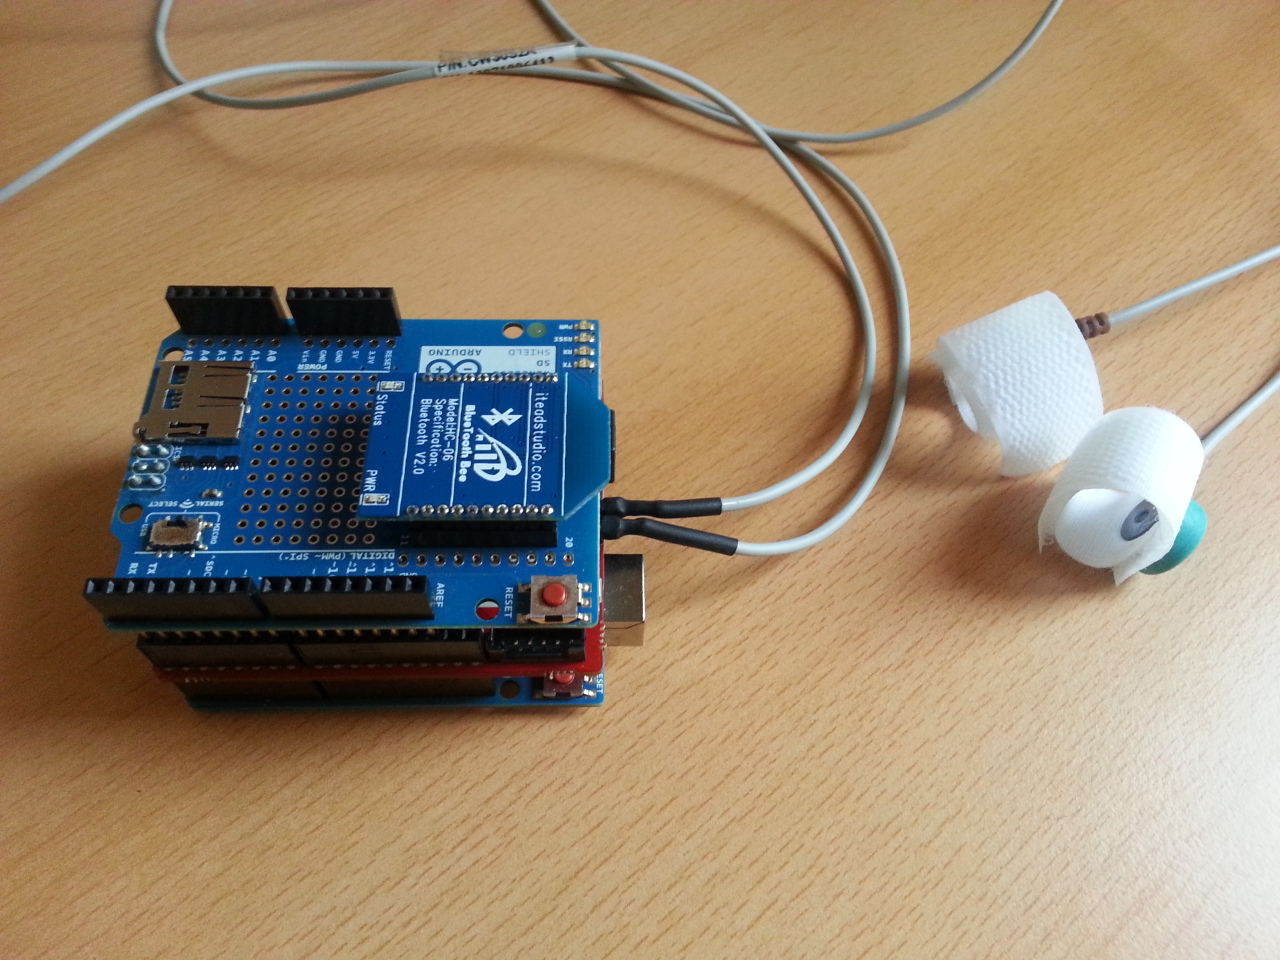
\includegraphics[width=0.7\textwidth]{implementierung_completestack.jpg}
	\caption{Der vollständige Stack}
	\label{fig:completeStack}
	\end{figure}
	
	
	\newpage
	\subsection{Android}
	
	Bei der Android-Entwicklung wurde auf eine Unterstützung mit \texttt{git} entwickelt. So konnte der Quellcode sowohl für Android- als auch Arduino- und LaTex-Quellcode versioniert verwaltet werden.
	
	\subsubsection{EEG: NeuroSky Brainwave Headset}
	
	Um das NeuroSky EEG Headset in Android anbinden zu können, bedarf es einiger Vorbereitungen:
	\begin{enumerate}
	\item Kauf und Download des Developer Tool für Android vom \href{http://store.neurosky.com/products/developer-tools-3-android} {NeuroSky Store}
	\item Erzeugen eines \texttt{lib}-Ordners im Android-Projekt, sofern nicht schon vorhanden
	\item Ablegen der \texttt{ThinkGear.jar}-Datei im lib-Ordner
	\item Importanweisung: ,,\texttt{import com.neurosky.thinkgear.*;}`` in der entsprechenden Activity
	\item AndroidManifest.xml: es ist die Bluetooth\_Permission zu setzen
	\end{enumerate}
	
	Des Weiteren müssen ein Android-BluetoothAdapter und ein TGDevice instanziiert werden.

	Der bluetoothAdapter wird mittels $BluetoothAdapter.getDefaultAdapter()$ zugewiesen. Wenn dieses erfolgreich war, dann wird das tgDevice erzeugt: \\* $tgDevice = new TGDevice(bluetoothAdapter, handler);$. Dem tgDevice wird der Default-BluetoothAdapter und eine $handler$ zugewiesen. 
	
	Der handler \label{handler} wird einer Handler-Class erzeugt. Dieser $handler$ hat die Aufgabe, Daten, die das Gerät sendet abzufangen und in einer gewünschten Form zu verarbeiten. Exemplarisch für die Aufmerksamkeitswerte des EEG:
	
	\begin{enumerate}
	\item case TGDevice.MSG\_ATTENTION:
    \item eeg\_att.setText('' Attention: " + msg.arg1 + "\textbackslash n" + eeg\_att.getText());
	\item break;
	\end{enumerate}
	
	Folgende Daten können vom EEG ausgelesen werden:
	
	\begin{itemize}
	\item Verbindungsstatus: STATE\_CONNECTING, STATE\_CONNECTED, \\STATE\_NOT\_FOUND, STATE\_NOTE\_PAIRED, STATE\_DISCONNECTED
	\item Auslesedaten: MSG\_ATTENTION, MSG\_Meditation, MSG\_BLINK, \\MSG\_HEART\_RATE
	\item sonstige Status: MSG\_LOW\_BATTERY, MSG\_POOR\_SIGNAL
	\end{itemize}
	
	Entscheidend für den Lügendetektor sind die Werte aus MSG\_ATTENTION, \\MSG\_MEDITATION und MSG\_BLINK. Anhand der Aufmerksamkeits- (attention) und Ruhewerte (meditation) kann man die Aufregung bzw. Entspannung bei der Testperson ablesen. Hinzu kommen die Augenblinzler (blink), die stark oder schwach ausgeprägt sein bzw. gezählt werden können und daher auf zusätzliches ,,unkontrolliertes`` / ,,nervöses`` Verhalten hinweisen.
	
	\begin{figure}[h!btp]
	\centering
	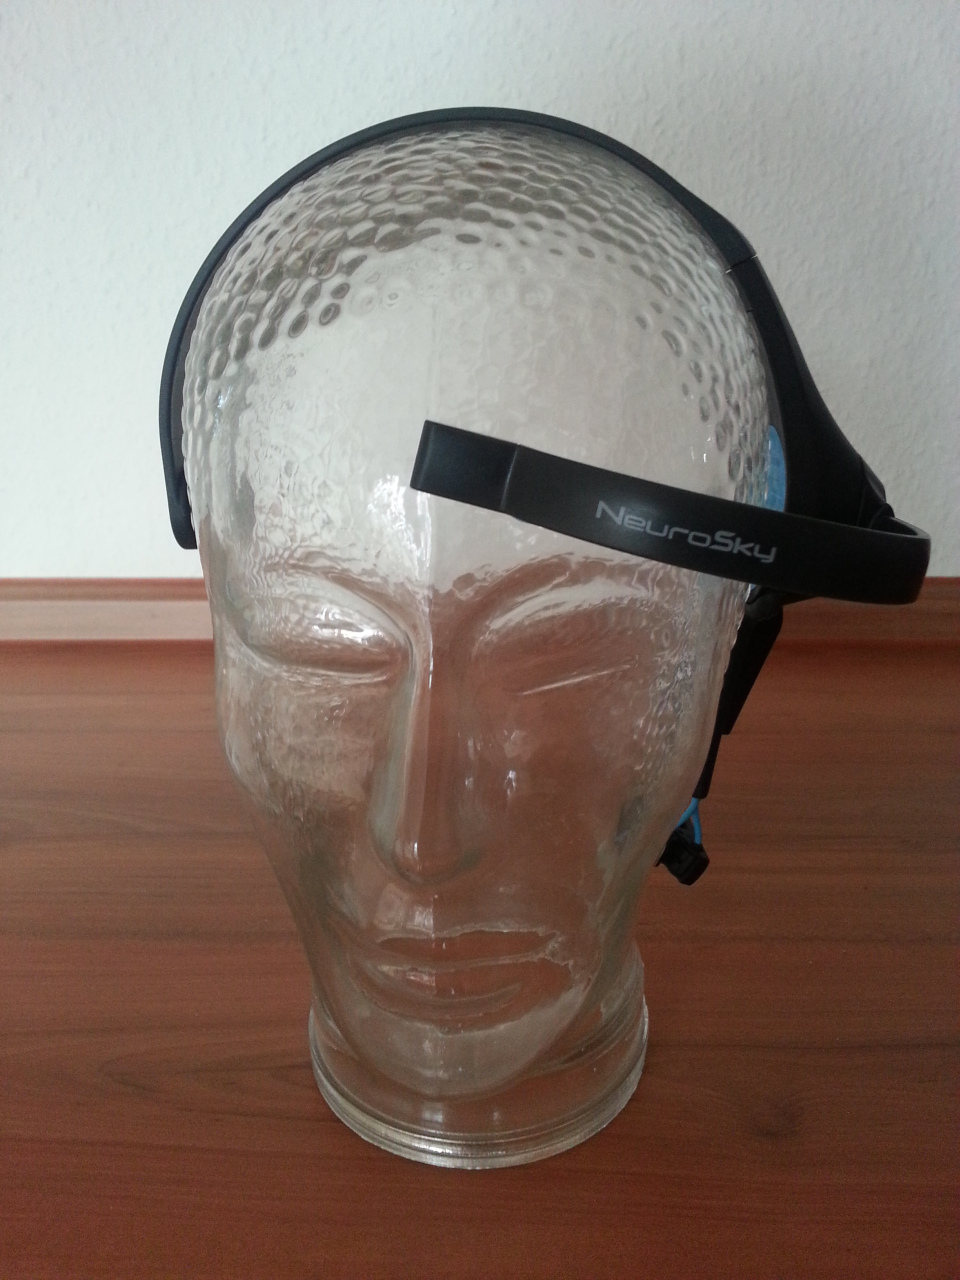
\includegraphics[width=0.5\textwidth]{implementierung_neuroskyheadset.jpg}
	\caption{Das NeuroSky Brainwave Headset}
	\label{fig:Brainwave-Headset}
	\end{figure}
	
	Das Anbinden des EEG an die Android-Applikation erfolgt über Bluetooth. Vor dem ersten Starten der Anwendung sollte das Android-Gerät mit dem EEG gepairt werden. Dann kann die eigene Anwendung gestartet werden. Sollte keine Verbindung in der Anwendung angezeigt werden, so sollte zusätzlich auf der EEG-Rückseite der ,,Pairing``-Knopf gedrückt werden.
	
	\subsubsection{Arduino Bluetooth}
			
	Zur Anbindung des Arduino Bluetooth Moduls kann man zweierlei vorgehen:
	\begin{enumerate}
	\item automatisierter (statischer) Verbindungsaufbau zwischen Android und Arduino
	\item dynamischer Verbindungsaufbau durch scannen vorhandener Bluetooth-Geräte
	\end{enumerate}
	
	Wir haben uns im Projekt dazu entschieden, dass wir die statische Methode wählen, da über das Scannen vorhandener Geräte der Verbindungsaufbau zu Fehlverbindungen geführt hatte und ggf. die Applikation geschlossen bzw. die built-in Bluetooth Funktionalität neugestartet werden musste. 
	
	Um die automatisierte Verbindung zu realisieren mussten eineige Vorbedingungen erfüllt werden:
	\begin{itemize}
	\item MAC-Adresse des Bluetooth-Moduls scannen
	\item MAC-Adresse in der Applikation hinterlegen
	\item SPP\footnote{serial port profile} UUID\footnote{128-bit universally unique identifier} für Verbindung festlegen\footnote{wird für Bluetooth Socket benötigt}
	\end{itemize}
	
	Zur Identifizierung des Arduino Bluetooth Moduls ,,linvor`` konnten wir mit der App $Power Bluetooth Scanner$ die MAC-Adresse ,,00:12:07:17:18:24`` auslesen. 
	Beim Aufbau der Bluetooth Verbindung soll eine UUID hinterlegt werden. Android (Google Inc.) selbst schlägt vor: ,,If you are connecting to a Bluetooth serial board then try using the well-known SPP UUID 00001101-0000-1000-8000-00805F9B34FB.``\footnote{http://developer.android.com/reference/android/bluetooth/BluetoothDevice.html}. 
	Auch für die Arduino Bluetooth zu Android Verbindung muss ein Handler erzeugt werden (vgl. EEG-Handler auf Seite \pageref{handler}).
	In diesem Fall musste der eingehende Datenstrom in ein byte-Array umgewandelt werden: $byte[] readBuf = (byte[]) msg.obj;$. Ausgehend von dem $msg.obj$ das über die seriellen Schnittstelle übertragen wird, können diese Signale in ein byte-Array gecastet und der Variable $readBuf$ zugewiesen werden. Aus dem byte-Array kann dann mittels $new String()$ ein String erzeugt und weiter verarbeitet werden.
	
	Die eigentliche Bluetooth-Verbindung wird in der $onResume()$ Methode hergestellt. Hierzu wird einer Variable btAdapter (von BluetoothAdapter, siehe EEG) durch die Methode $create BluetoothSocket(device)$ gesetzt. 
	Der Parameter device ist eben die Verbindung (über die MAC-Adresse) zum Ardunio Bluetooth Shield \\ \\
	$BluetoothDevice$ $device = btAdapter.getRemoteDevice(ADDRESS);$\\ \\
	Mit der Erstellung des Bluetooth-Socket kann nun ein Verbindungs-Thread (ConnectedThread) erzeugt werden. Dieser sorgt dafür, dass die eingehenden Daten ordnungsgemäß (ge'threaded') empfangen (wenn gewünscht auch gesendet) werden können. 
	
	Mit $mConnectedThread = new ConnectedThread(btSocket);$ und \\$mConnectedThread.start();$ wird der Thread gestartet.
	
	\subsubsection*{Bluetooth-Status überprüfen}
	
	Da eine gültige Verbindung nur mit angeschaltetem Bluetooth-Modul des mobilen Geräts funktioniert, muss von der Anwendung überprüft werden, ob Bluetooth angeschaltet ist. Dazu wird die Methode \texttt{checkBTState()} genutzt. Sie wird in der Activity-Methode \texttt{onCreate()} gestartet und überprüft folgende Status:
	\begin{enumerate}
	\item wurde ein Bluetooth-Adapter angelegt, wenn nicht, dann beende und gib Fehlermeldung aus
	\item Bluetooth-Adapter vorhanden und ,,enabled``, dann ist alles ok
	\item Bluetooth-Adapter vorhanden aber nicht ,,enabled``, dann erzeuge und rufe einen Intent mit $BluetoothAdapter.ACTION\_REQUEST\_ENABLE$ auf und starte die Methode $startActivityForResult()$ um das Anschalten des Bluetooth-Mo-duls zu erzwingen.
	\end{enumerate}
		
	\subsubsection{Spielaufbau}
	
	
	\subsubsection*{Die Spiellogik}
	
	Die Logik des Spiels setzt sich aus den Parameter:
	\begin{enumerate}
	\item Attention: Aufmerksamkeit
	\item Meditation: Ruhewert
	\item Blinks: Augenblinzeln
	\item Galvanic: Hautwiderstand
	\end{enumerate}
	
zusammen.
Für jede Frage wird für jeden o.g. Parameter ein int-Array erzeugt. 
Dieses Array wird pro Sekunde mit den aktuellen Werten des Sensors gefüllt. 
Für die Aufmerksamkeits-, Ruhewert- und Hautwiderstandswerte wird im Anschluss die Standardabweichung gebildet. 
Diese entscheidet darüber, ob es Änderungen im Bereich der gemessenen Sensordaten gibt oder nicht. 
Vor jeder neuen Fragerunde wird für die Spieler eine Kalibrierung durchgeführt. 
Diese Kalibrierung ermittelt jeweils einen Referenzwert für die Aufmerksamkeits-, Ruhewert- und Hautwiderstandswerte. 
Nach jeder Frage kann dann überprüft werden, ob die neu berechneten Standardabweichungen für Aufmerksamkeits-, Ruhewert- und Hautwiderstandswerte mit den Referenzwerten aus der Kalibrierung übereinstimmen oder in einem Bereich von - bis liegen. 
Sollten die neuen Werte über den Grenzwerten liegen, so wird eine Lüge (erhöhte Anspannung) vermutet.

Zusätzlich werden für jede Runde die Anzahl der Augenblinzler gezählt. 
Auch diese werden während der Kalibrierung gezählt und im Anschluss bei jeder Frage verglichen. 
Gerade wenn mehr Augenblinzler in einer Fragerunde gezählt werden wie im Vergleich zur Kalibrierung, so kann man von einer Lüge sprechen.

Alle vier Parameter werden dann in einer Methode miteinanderverglichen.
Die Methode liefert dann entsprechend einen boolschen Wert (true/false) zurück, ob eine Lüge vorliegt oder nicht.
	
	\subsubsection{Datenpersistenz}
	
	
	\subsubsection{Datenvisualisierung}

	\newpage
\section{Verifizierung, Evaluation}
	   	\section{Geschäftsmodell}
   	Zur Beschreibung der Funktionsweise des zukünftigen Unternehmens und Evaluierung der optimalen Gewinnerwirtschaftung wurden drei Business Model Canvas erstellt. Dabei wurden die im Kapitel Personas und Anwendungsszenarien beschriebenen Zielgruppen betrachtet.

   	\begin{landscape}
	\newpage
	\subsection{Business Model Canvas - Persona-Typ: Wissenschaftler}
   	\begin{table}[h!]
		\begin{center}
			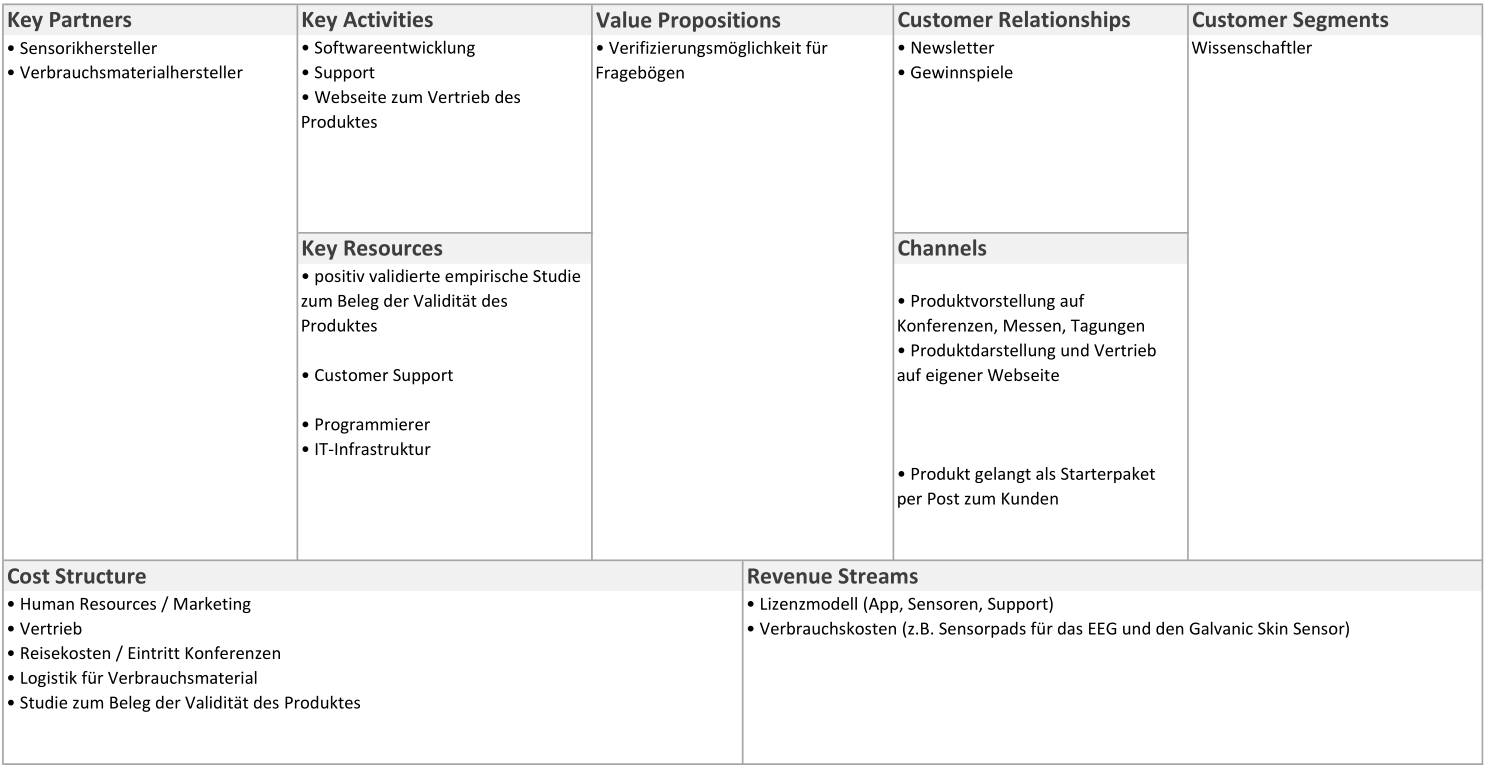
\includegraphics[width=1.3\textwidth]{business_canvas_1_wissenschftler.png}
		\end{center}
		\caption[Business Model Canvas - Persona-Typ: Wissenschaftler]{Business Model Canvas für die Persona vom Typ Wissenschaftler}
		\label{fig:business_model_1}
	\end{table}
	
	\newpage
   	\subsection{Business Model Canvas - Persona-Typ: Angeber}
   	\begin{table}[h!]
		\begin{center}
			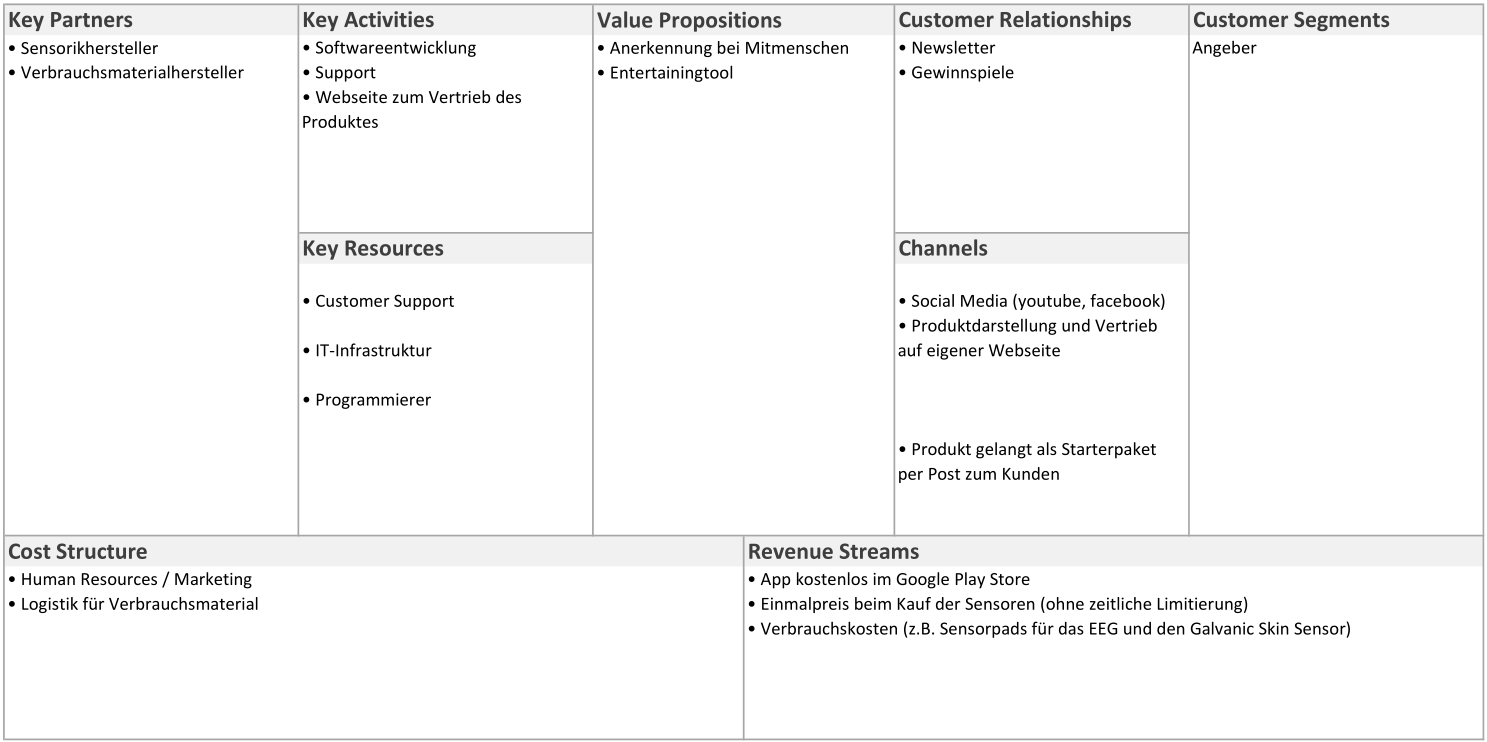
\includegraphics[width=1.3\textwidth]{business_canvas_2_angeber.png}
		\end{center}
		\caption[Business Model Canvas - Persona-Typ: Angeber]{Business Model Canvas für die Persona vom Typ Angeber}
		\label{fig:business_model_2}
	\end{table}
	
	\newpage
	\subsection{Business Model Canvas - Persona-Typ: Kontrollfreak}
   	\begin{table}[h!]
		\begin{center}
			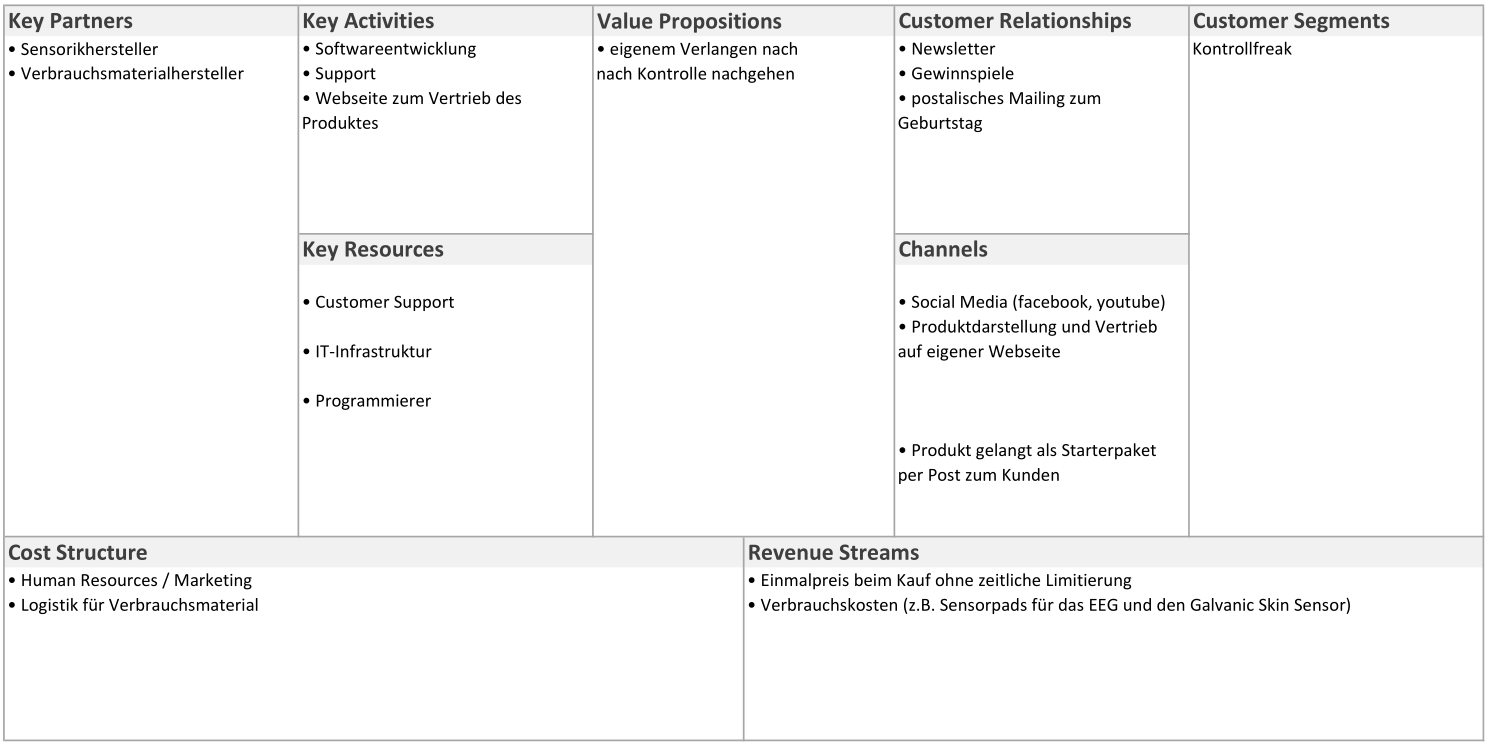
\includegraphics[width=1.3\textwidth]{business_canvas_3_kontrollfreak.png}
		\end{center}
		\caption[Business Model Canvas - Persona-Typ: Kontrollfreak]{Business Model Canvas für die Persona vom Typ Kontrollfreak}
		\label{fig:business_model_3}
	\end{table}

	\newpage
	\subsection{Fazit zum Geschäftsmodell}
	Als Fazit ergab sich, dass der Persona-Typ Wissenschaftler ein deutlich erhöhtes Ausmaß an Investitionen, wie beispielsweise Kosten für eine Studie zum Beleg der Validität des Produktes, benötigt. Da zudem Beschaffungsprozesse an der Universität einen langen Zeitraum andauern können, ergibt sich für das Unternehmen ein hoher finanzieller Aufwand und eine längere Zeit ohne Einnahmen. Dies ergibt ein hohes Risiko für unser Unternehmen und aus diesem Grund schließen wir dieses Geschäftsmodell aus. Der Persona-Typ Angeber kann nicht langfristig an unser Produkt gebunden werden und scheidet aus diesem Grund ebenfalls als Geschäftsmodell aus. Wir haben uns für eine Spezialisierung auf den Persona-Typ Kontrollfreak entschieden, da eine langfristige Bindung an unser Produkt und geringere Anfangskosten als beim Persona-Typ Wissenschaftler zu erwarten sind.

   	\begin{table}[h!]
		\begin{center}
			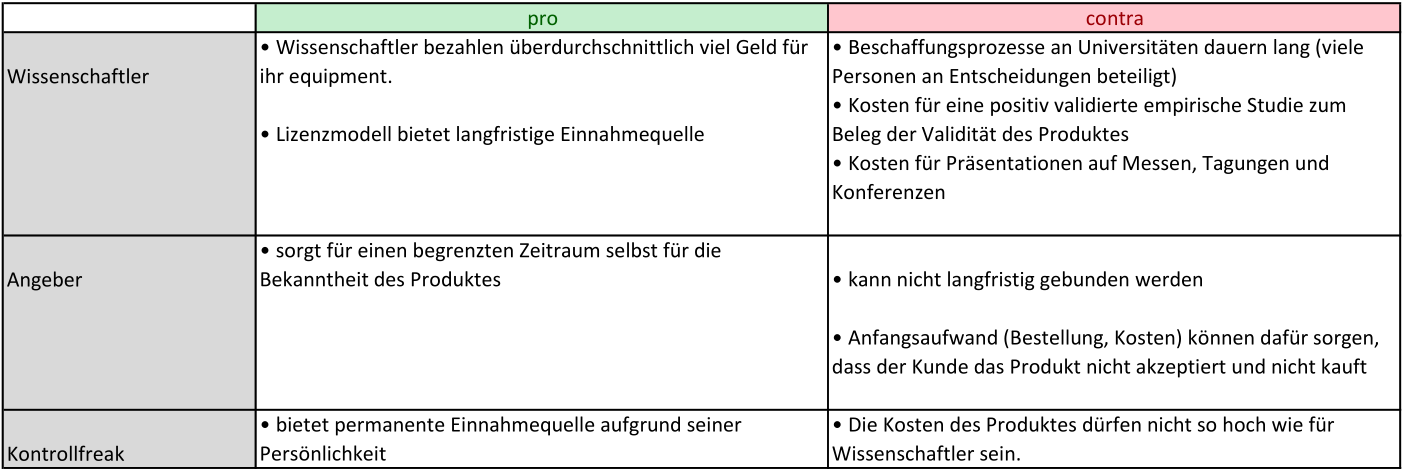
\includegraphics[width=1.1\textwidth]{business_canvas_4_pro_contra.png}
		\end{center}
		\caption[Business Model Canvas - Pro/Contra Auswertung]{Pro/Contra Auswertung der Business Model Canvas}
		\label{fig:business_model_2}
	\end{table}
	\end{landscape}

\end{document}
